% Options for packages loaded elsewhere
\PassOptionsToPackage{unicode}{hyperref}
\PassOptionsToPackage{hyphens}{url}
%
\documentclass[
  english,
  man,floatsintext]{apa6}
\usepackage{lmodern}
\usepackage{amsmath}
\usepackage{ifxetex,ifluatex}
\ifnum 0\ifxetex 1\fi\ifluatex 1\fi=0 % if pdftex
  \usepackage[T1]{fontenc}
  \usepackage[utf8]{inputenc}
  \usepackage{textcomp} % provide euro and other symbols
  \usepackage{amssymb}
\else % if luatex or xetex
  \usepackage{unicode-math}
  \defaultfontfeatures{Scale=MatchLowercase}
  \defaultfontfeatures[\rmfamily]{Ligatures=TeX,Scale=1}
\fi
% Use upquote if available, for straight quotes in verbatim environments
\IfFileExists{upquote.sty}{\usepackage{upquote}}{}
\IfFileExists{microtype.sty}{% use microtype if available
  \usepackage[]{microtype}
  \UseMicrotypeSet[protrusion]{basicmath} % disable protrusion for tt fonts
}{}
\makeatletter
\@ifundefined{KOMAClassName}{% if non-KOMA class
  \IfFileExists{parskip.sty}{%
    \usepackage{parskip}
  }{% else
    \setlength{\parindent}{0pt}
    \setlength{\parskip}{6pt plus 2pt minus 1pt}}
}{% if KOMA class
  \KOMAoptions{parskip=half}}
\makeatother
\usepackage{xcolor}
\IfFileExists{xurl.sty}{\usepackage{xurl}}{} % add URL line breaks if available
\IfFileExists{bookmark.sty}{\usepackage{bookmark}}{\usepackage{hyperref}}
\hypersetup{
  pdftitle={EDLD651 Final Project},
  pdfauthor={Maggie Head1, Sarah Spafford1, \& Heather Terral1},
  pdflang={en-EN},
  pdfkeywords={keywords},
  hidelinks,
  pdfcreator={LaTeX via pandoc}}
\urlstyle{same} % disable monospaced font for URLs
\usepackage{longtable,booktabs}
% Correct order of tables after \paragraph or \subparagraph
\usepackage{etoolbox}
\makeatletter
\patchcmd\longtable{\par}{\if@noskipsec\mbox{}\fi\par}{}{}
\makeatother
% Allow footnotes in longtable head/foot
\IfFileExists{footnotehyper.sty}{\usepackage{footnotehyper}}{\usepackage{footnote}}
\makesavenoteenv{longtable}
\usepackage{graphicx}
\makeatletter
\def\maxwidth{\ifdim\Gin@nat@width>\linewidth\linewidth\else\Gin@nat@width\fi}
\def\maxheight{\ifdim\Gin@nat@height>\textheight\textheight\else\Gin@nat@height\fi}
\makeatother
% Scale images if necessary, so that they will not overflow the page
% margins by default, and it is still possible to overwrite the defaults
% using explicit options in \includegraphics[width, height, ...]{}
\setkeys{Gin}{width=\maxwidth,height=\maxheight,keepaspectratio}
% Set default figure placement to htbp
\makeatletter
\def\fps@figure{htbp}
\makeatother
\setlength{\emergencystretch}{3em} % prevent overfull lines
\providecommand{\tightlist}{%
  \setlength{\itemsep}{0pt}\setlength{\parskip}{0pt}}
\setcounter{secnumdepth}{-\maxdimen} % remove section numbering
% Make \paragraph and \subparagraph free-standing
\ifx\paragraph\undefined\else
  \let\oldparagraph\paragraph
  \renewcommand{\paragraph}[1]{\oldparagraph{#1}\mbox{}}
\fi
\ifx\subparagraph\undefined\else
  \let\oldsubparagraph\subparagraph
  \renewcommand{\subparagraph}[1]{\oldsubparagraph{#1}\mbox{}}
\fi
% Manuscript styling
\usepackage{upgreek}
\captionsetup{font=singlespacing,justification=justified}

% Table formatting
\usepackage{longtable}
\usepackage{lscape}
% \usepackage[counterclockwise]{rotating}   % Landscape page setup for large tables
\usepackage{multirow}		% Table styling
\usepackage{tabularx}		% Control Column width
\usepackage[flushleft]{threeparttable}	% Allows for three part tables with a specified notes section
\usepackage{threeparttablex}            % Lets threeparttable work with longtable

% Create new environments so endfloat can handle them
% \newenvironment{ltable}
%   {\begin{landscape}\begin{center}\begin{threeparttable}}
%   {\end{threeparttable}\end{center}\end{landscape}}
\newenvironment{lltable}{\begin{landscape}\begin{center}\begin{ThreePartTable}}{\end{ThreePartTable}\end{center}\end{landscape}}

% Enables adjusting longtable caption width to table width
% Solution found at http://golatex.de/longtable-mit-caption-so-breit-wie-die-tabelle-t15767.html
\makeatletter
\newcommand\LastLTentrywidth{1em}
\newlength\longtablewidth
\setlength{\longtablewidth}{1in}
\newcommand{\getlongtablewidth}{\begingroup \ifcsname LT@\roman{LT@tables}\endcsname \global\longtablewidth=0pt \renewcommand{\LT@entry}[2]{\global\advance\longtablewidth by ##2\relax\gdef\LastLTentrywidth{##2}}\@nameuse{LT@\roman{LT@tables}} \fi \endgroup}

% \setlength{\parindent}{0.5in}
% \setlength{\parskip}{0pt plus 0pt minus 0pt}

% \usepackage{etoolbox}
\makeatletter
\patchcmd{\HyOrg@maketitle}
  {\section{\normalfont\normalsize\abstractname}}
  {\section*{\normalfont\normalsize\abstractname}}
  {}{\typeout{Failed to patch abstract.}}
\patchcmd{\HyOrg@maketitle}
  {\section{\protect\normalfont{\@title}}}
  {\section*{\protect\normalfont{\@title}}}
  {}{\typeout{Failed to patch title.}}
\makeatother
\shorttitle{Title}
\keywords{keywords\newline\indent Word count: X}
\usepackage{lineno}

\linenumbers
\usepackage{csquotes}
\ifxetex
  % Load polyglossia as late as possible: uses bidi with RTL langages (e.g. Hebrew, Arabic)
  \usepackage{polyglossia}
  \setmainlanguage[]{english}
\else
  \usepackage[shorthands=off,main=english]{babel}
\fi
\ifluatex
  \usepackage{selnolig}  % disable illegal ligatures
\fi
\usepackage[]{biblatex}
\addbibresource{r-references.bib}
\newlength{\cslhangindent}
\setlength{\cslhangindent}{1.5em}
\newlength{\csllabelwidth}
\setlength{\csllabelwidth}{3em}
\newenvironment{CSLReferences}[3] % #1 hanging-ident, #2 entry spacing
 {% don't indent paragraphs
  \setlength{\parindent}{0pt}
  % turn on hanging indent if param 1 is 1
  \ifodd #1 \everypar{\setlength{\hangindent}{\cslhangindent}}\ignorespaces\fi
  % set entry spacing
  \ifnum #2 > 0
  \setlength{\parskip}{#2\baselineskip}
  \fi
 }%
 {}
\usepackage{calc} % for \widthof, \maxof
\newcommand{\CSLBlock}[1]{#1\hfill\break}
\newcommand{\CSLLeftMargin}[1]{\parbox[t]{\maxof{\widthof{#1}}{\csllabelwidth}}{#1}}
\newcommand{\CSLRightInline}[1]{\parbox[t]{\linewidth}{#1}}
\newcommand{\CSLIndent}[1]{\hspace{\cslhangindent}#1}

\title{EDLD651 Final Project}
\author{Maggie Head\textsuperscript{1}, Sarah Spafford\textsuperscript{1}, \& Heather Terral\textsuperscript{1}}
\date{}


\authornote{

This will be an author note.

Enter author note here.

The authors made the following contributions. Maggie Head: Conceptualization, Writing - Original Draft Preparation, Writing - Review \& Editing; Sarah Spafford: Writing - Review \& Editing; Heather Terral: Writing - Review \& Editing.

Correspondence concerning this article should be addressed to Maggie Head, Postal address. E-mail: \href{mailto:my@email.com}{\nolinkurl{my@email.com}}

}

\affiliation{\vspace{0.5cm}\textsuperscript{1} University of Oregon}

\abstract{
This will be an abstract.
}



\begin{document}
\maketitle

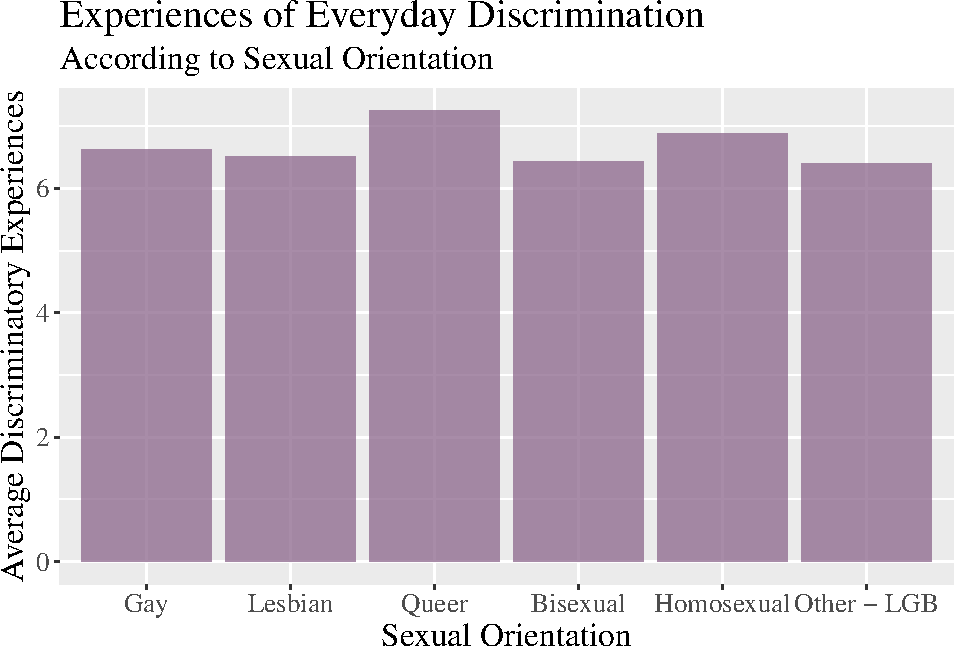
\includegraphics{prep_script_files/figure-latex/mean plot-1.pdf}

\begin{longtable}[]{@{}ll@{}}
\toprule
& stridy (N = 396)\tabularnewline
\midrule
\endhead
\textbf{Everyday Discrmination} & ~~\tabularnewline
~~ min & 0\tabularnewline
~~ median & 7\tabularnewline
~~ max & 8\tabularnewline
~~ mean (sd) & 6.56 ± 1.93\tabularnewline
\textbf{Chronic Strain} & ~~\tabularnewline
~~ min & 1\tabularnewline
~~ median & 1.67\tabularnewline
~~ max & 3\tabularnewline
~~ mean (sd) & 371; 1.72 ± 0.54\tabularnewline
\textbf{Psychological Wellbeing} & ~~\tabularnewline
~~ min & 3\tabularnewline
~~ median & 5.56\tabularnewline
~~ max & 7\tabularnewline
~~ mean (sd) & 366; 5.46 ± 0.79\tabularnewline
\textbf{Social Connectedness} & ~~\tabularnewline
~~ min & 1.38\tabularnewline
~~ median & 3.38\tabularnewline
~~ max & 4\tabularnewline
~~ mean (sd) & 390; 3.30 ± 0.52\tabularnewline
\bottomrule
\end{longtable}

\begin{longtable}[]{@{}lllllll@{}}
\toprule
\begin{minipage}[b]{0.14\columnwidth}\raggedright
\strut
\end{minipage} & \begin{minipage}[b]{0.11\columnwidth}\raggedright
Bisexual (N = 71)\strut
\end{minipage} & \begin{minipage}[b]{0.12\columnwidth}\raggedright
Gay (N = 178)\strut
\end{minipage} & \begin{minipage}[b]{0.10\columnwidth}\raggedright
Homosexual (N = 16)\strut
\end{minipage} & \begin{minipage}[b]{0.12\columnwidth}\raggedright
Lesbian (N = 111)\strut
\end{minipage} & \begin{minipage}[b]{0.10\columnwidth}\raggedright
Other - LGB (N = 5)\strut
\end{minipage} & \begin{minipage}[b]{0.11\columnwidth}\raggedright
Queer (N = 15)\strut
\end{minipage}\tabularnewline
\midrule
\endhead
\begin{minipage}[t]{0.14\columnwidth}\raggedright
\textbf{Everyday Discrmination}\strut
\end{minipage} & \begin{minipage}[t]{0.11\columnwidth}\raggedright
~~\strut
\end{minipage} & \begin{minipage}[t]{0.12\columnwidth}\raggedright
~~\strut
\end{minipage} & \begin{minipage}[t]{0.10\columnwidth}\raggedright
~~\strut
\end{minipage} & \begin{minipage}[t]{0.12\columnwidth}\raggedright
~~\strut
\end{minipage} & \begin{minipage}[t]{0.10\columnwidth}\raggedright
~~\strut
\end{minipage} & \begin{minipage}[t]{0.11\columnwidth}\raggedright
~~\strut
\end{minipage}\tabularnewline
\begin{minipage}[t]{0.14\columnwidth}\raggedright
~~ min\strut
\end{minipage} & \begin{minipage}[t]{0.11\columnwidth}\raggedright
0\strut
\end{minipage} & \begin{minipage}[t]{0.12\columnwidth}\raggedright
0\strut
\end{minipage} & \begin{minipage}[t]{0.10\columnwidth}\raggedright
0\strut
\end{minipage} & \begin{minipage}[t]{0.12\columnwidth}\raggedright
0\strut
\end{minipage} & \begin{minipage}[t]{0.10\columnwidth}\raggedright
5\strut
\end{minipage} & \begin{minipage}[t]{0.11\columnwidth}\raggedright
0\strut
\end{minipage}\tabularnewline
\begin{minipage}[t]{0.14\columnwidth}\raggedright
~~ median\strut
\end{minipage} & \begin{minipage}[t]{0.11\columnwidth}\raggedright
7\strut
\end{minipage} & \begin{minipage}[t]{0.12\columnwidth}\raggedright
7\strut
\end{minipage} & \begin{minipage}[t]{0.10\columnwidth}\raggedright
8\strut
\end{minipage} & \begin{minipage}[t]{0.12\columnwidth}\raggedright
7\strut
\end{minipage} & \begin{minipage}[t]{0.10\columnwidth}\raggedright
6\strut
\end{minipage} & \begin{minipage}[t]{0.11\columnwidth}\raggedright
7\strut
\end{minipage}\tabularnewline
\begin{minipage}[t]{0.14\columnwidth}\raggedright
~~ max\strut
\end{minipage} & \begin{minipage}[t]{0.11\columnwidth}\raggedright
8\strut
\end{minipage} & \begin{minipage}[t]{0.12\columnwidth}\raggedright
8\strut
\end{minipage} & \begin{minipage}[t]{0.10\columnwidth}\raggedright
8\strut
\end{minipage} & \begin{minipage}[t]{0.12\columnwidth}\raggedright
8\strut
\end{minipage} & \begin{minipage}[t]{0.10\columnwidth}\raggedright
8\strut
\end{minipage} & \begin{minipage}[t]{0.11\columnwidth}\raggedright
8\strut
\end{minipage}\tabularnewline
\begin{minipage}[t]{0.14\columnwidth}\raggedright
~~ mean (sd)\strut
\end{minipage} & \begin{minipage}[t]{0.11\columnwidth}\raggedright
6.38 ± 2.20\strut
\end{minipage} & \begin{minipage}[t]{0.12\columnwidth}\raggedright
6.65 ± 1.75\strut
\end{minipage} & \begin{minipage}[t]{0.10\columnwidth}\raggedright
6.88 ± 2.03\strut
\end{minipage} & \begin{minipage}[t]{0.12\columnwidth}\raggedright
6.45 ± 2.03\strut
\end{minipage} & \begin{minipage}[t]{0.10\columnwidth}\raggedright
6.40 ± 1.14\strut
\end{minipage} & \begin{minipage}[t]{0.11\columnwidth}\raggedright
6.80 ± 2.04\strut
\end{minipage}\tabularnewline
\begin{minipage}[t]{0.14\columnwidth}\raggedright
\textbf{Chronic Strain}\strut
\end{minipage} & \begin{minipage}[t]{0.11\columnwidth}\raggedright
~~\strut
\end{minipage} & \begin{minipage}[t]{0.12\columnwidth}\raggedright
~~\strut
\end{minipage} & \begin{minipage}[t]{0.10\columnwidth}\raggedright
~~\strut
\end{minipage} & \begin{minipage}[t]{0.12\columnwidth}\raggedright
~~\strut
\end{minipage} & \begin{minipage}[t]{0.10\columnwidth}\raggedright
~~\strut
\end{minipage} & \begin{minipage}[t]{0.11\columnwidth}\raggedright
~~\strut
\end{minipage}\tabularnewline
\begin{minipage}[t]{0.14\columnwidth}\raggedright
~~ min\strut
\end{minipage} & \begin{minipage}[t]{0.11\columnwidth}\raggedright
1\strut
\end{minipage} & \begin{minipage}[t]{0.12\columnwidth}\raggedright
1\strut
\end{minipage} & \begin{minipage}[t]{0.10\columnwidth}\raggedright
1\strut
\end{minipage} & \begin{minipage}[t]{0.12\columnwidth}\raggedright
1\strut
\end{minipage} & \begin{minipage}[t]{0.10\columnwidth}\raggedright
1.33\strut
\end{minipage} & \begin{minipage}[t]{0.11\columnwidth}\raggedright
1\strut
\end{minipage}\tabularnewline
\begin{minipage}[t]{0.14\columnwidth}\raggedright
~~ median\strut
\end{minipage} & \begin{minipage}[t]{0.11\columnwidth}\raggedright
2\strut
\end{minipage} & \begin{minipage}[t]{0.12\columnwidth}\raggedright
1.67\strut
\end{minipage} & \begin{minipage}[t]{0.10\columnwidth}\raggedright
1.33\strut
\end{minipage} & \begin{minipage}[t]{0.12\columnwidth}\raggedright
1.67\strut
\end{minipage} & \begin{minipage}[t]{0.10\columnwidth}\raggedright
2\strut
\end{minipage} & \begin{minipage}[t]{0.11\columnwidth}\raggedright
1.33\strut
\end{minipage}\tabularnewline
\begin{minipage}[t]{0.14\columnwidth}\raggedright
~~ max\strut
\end{minipage} & \begin{minipage}[t]{0.11\columnwidth}\raggedright
2.67\strut
\end{minipage} & \begin{minipage}[t]{0.12\columnwidth}\raggedright
3\strut
\end{minipage} & \begin{minipage}[t]{0.10\columnwidth}\raggedright
1.67\strut
\end{minipage} & \begin{minipage}[t]{0.12\columnwidth}\raggedright
3\strut
\end{minipage} & \begin{minipage}[t]{0.10\columnwidth}\raggedright
2.67\strut
\end{minipage} & \begin{minipage}[t]{0.11\columnwidth}\raggedright
3\strut
\end{minipage}\tabularnewline
\begin{minipage}[t]{0.14\columnwidth}\raggedright
~~ mean (sd)\strut
\end{minipage} & \begin{minipage}[t]{0.11\columnwidth}\raggedright
67; 1.88 ± 0.49\strut
\end{minipage} & \begin{minipage}[t]{0.12\columnwidth}\raggedright
166; 1.67 ± 0.54\strut
\end{minipage} & \begin{minipage}[t]{0.10\columnwidth}\raggedright
1.35 ± 0.26\strut
\end{minipage} & \begin{minipage}[t]{0.12\columnwidth}\raggedright
104; 1.77 ± 0.58\strut
\end{minipage} & \begin{minipage}[t]{0.10\columnwidth}\raggedright
1.87 ± 0.56\strut
\end{minipage} & \begin{minipage}[t]{0.11\columnwidth}\raggedright
13; 1.62 ± 0.59\strut
\end{minipage}\tabularnewline
\begin{minipage}[t]{0.14\columnwidth}\raggedright
\textbf{Psychological Wellbeing}\strut
\end{minipage} & \begin{minipage}[t]{0.11\columnwidth}\raggedright
~~\strut
\end{minipage} & \begin{minipage}[t]{0.12\columnwidth}\raggedright
~~\strut
\end{minipage} & \begin{minipage}[t]{0.10\columnwidth}\raggedright
~~\strut
\end{minipage} & \begin{minipage}[t]{0.12\columnwidth}\raggedright
~~\strut
\end{minipage} & \begin{minipage}[t]{0.10\columnwidth}\raggedright
~~\strut
\end{minipage} & \begin{minipage}[t]{0.11\columnwidth}\raggedright
~~\strut
\end{minipage}\tabularnewline
\begin{minipage}[t]{0.14\columnwidth}\raggedright
~~ min\strut
\end{minipage} & \begin{minipage}[t]{0.11\columnwidth}\raggedright
3.18\strut
\end{minipage} & \begin{minipage}[t]{0.12\columnwidth}\raggedright
3\strut
\end{minipage} & \begin{minipage}[t]{0.10\columnwidth}\raggedright
3.12\strut
\end{minipage} & \begin{minipage}[t]{0.12\columnwidth}\raggedright
3.41\strut
\end{minipage} & \begin{minipage}[t]{0.10\columnwidth}\raggedright
3.88\strut
\end{minipage} & \begin{minipage}[t]{0.11\columnwidth}\raggedright
4.29\strut
\end{minipage}\tabularnewline
\begin{minipage}[t]{0.14\columnwidth}\raggedright
~~ median\strut
\end{minipage} & \begin{minipage}[t]{0.11\columnwidth}\raggedright
5.24\strut
\end{minipage} & \begin{minipage}[t]{0.12\columnwidth}\raggedright
5.59\strut
\end{minipage} & \begin{minipage}[t]{0.10\columnwidth}\raggedright
5.74\strut
\end{minipage} & \begin{minipage}[t]{0.12\columnwidth}\raggedright
5.53\strut
\end{minipage} & \begin{minipage}[t]{0.10\columnwidth}\raggedright
5.12\strut
\end{minipage} & \begin{minipage}[t]{0.11\columnwidth}\raggedright
6\strut
\end{minipage}\tabularnewline
\begin{minipage}[t]{0.14\columnwidth}\raggedright
~~ max\strut
\end{minipage} & \begin{minipage}[t]{0.11\columnwidth}\raggedright
6.82\strut
\end{minipage} & \begin{minipage}[t]{0.12\columnwidth}\raggedright
7\strut
\end{minipage} & \begin{minipage}[t]{0.10\columnwidth}\raggedright
6.59\strut
\end{minipage} & \begin{minipage}[t]{0.12\columnwidth}\raggedright
6.82\strut
\end{minipage} & \begin{minipage}[t]{0.10\columnwidth}\raggedright
5.76\strut
\end{minipage} & \begin{minipage}[t]{0.11\columnwidth}\raggedright
7\strut
\end{minipage}\tabularnewline
\begin{minipage}[t]{0.14\columnwidth}\raggedright
~~ mean (sd)\strut
\end{minipage} & \begin{minipage}[t]{0.11\columnwidth}\raggedright
64; 5.23 ± 0.86\strut
\end{minipage} & \begin{minipage}[t]{0.12\columnwidth}\raggedright
164; 5.51 ± 0.78\strut
\end{minipage} & \begin{minipage}[t]{0.10\columnwidth}\raggedright
5.47 ± 1.01\strut
\end{minipage} & \begin{minipage}[t]{0.12\columnwidth}\raggedright
104; 5.53 ± 0.70\strut
\end{minipage} & \begin{minipage}[t]{0.10\columnwidth}\raggedright
4.95 ± 0.72\strut
\end{minipage} & \begin{minipage}[t]{0.11\columnwidth}\raggedright
13; 5.68 ± 0.79\strut
\end{minipage}\tabularnewline
\begin{minipage}[t]{0.14\columnwidth}\raggedright
\textbf{Social Connectedness}\strut
\end{minipage} & \begin{minipage}[t]{0.11\columnwidth}\raggedright
~~\strut
\end{minipage} & \begin{minipage}[t]{0.12\columnwidth}\raggedright
~~\strut
\end{minipage} & \begin{minipage}[t]{0.10\columnwidth}\raggedright
~~\strut
\end{minipage} & \begin{minipage}[t]{0.12\columnwidth}\raggedright
~~\strut
\end{minipage} & \begin{minipage}[t]{0.10\columnwidth}\raggedright
~~\strut
\end{minipage} & \begin{minipage}[t]{0.11\columnwidth}\raggedright
~~\strut
\end{minipage}\tabularnewline
\begin{minipage}[t]{0.14\columnwidth}\raggedright
~~ min\strut
\end{minipage} & \begin{minipage}[t]{0.11\columnwidth}\raggedright
1.62\strut
\end{minipage} & \begin{minipage}[t]{0.12\columnwidth}\raggedright
1.38\strut
\end{minipage} & \begin{minipage}[t]{0.10\columnwidth}\raggedright
2.62\strut
\end{minipage} & \begin{minipage}[t]{0.12\columnwidth}\raggedright
2.12\strut
\end{minipage} & \begin{minipage}[t]{0.10\columnwidth}\raggedright
2.12\strut
\end{minipage} & \begin{minipage}[t]{0.11\columnwidth}\raggedright
3.25\strut
\end{minipage}\tabularnewline
\begin{minipage}[t]{0.14\columnwidth}\raggedright
~~ median\strut
\end{minipage} & \begin{minipage}[t]{0.11\columnwidth}\raggedright
3.12\strut
\end{minipage} & \begin{minipage}[t]{0.12\columnwidth}\raggedright
3.38\strut
\end{minipage} & \begin{minipage}[t]{0.10\columnwidth}\raggedright
3.5\strut
\end{minipage} & \begin{minipage}[t]{0.12\columnwidth}\raggedright
3.5\strut
\end{minipage} & \begin{minipage}[t]{0.10\columnwidth}\raggedright
2.75\strut
\end{minipage} & \begin{minipage}[t]{0.11\columnwidth}\raggedright
3.5\strut
\end{minipage}\tabularnewline
\begin{minipage}[t]{0.14\columnwidth}\raggedright
~~ max\strut
\end{minipage} & \begin{minipage}[t]{0.11\columnwidth}\raggedright
4\strut
\end{minipage} & \begin{minipage}[t]{0.12\columnwidth}\raggedright
4\strut
\end{minipage} & \begin{minipage}[t]{0.10\columnwidth}\raggedright
3.88\strut
\end{minipage} & \begin{minipage}[t]{0.12\columnwidth}\raggedright
4\strut
\end{minipage} & \begin{minipage}[t]{0.10\columnwidth}\raggedright
3.75\strut
\end{minipage} & \begin{minipage}[t]{0.11\columnwidth}\raggedright
4\strut
\end{minipage}\tabularnewline
\begin{minipage}[t]{0.14\columnwidth}\raggedright
~~ mean (sd)\strut
\end{minipage} & \begin{minipage}[t]{0.11\columnwidth}\raggedright
70; 3.11 ± 0.53\strut
\end{minipage} & \begin{minipage}[t]{0.12\columnwidth}\raggedright
174; 3.29 ± 0.53\strut
\end{minipage} & \begin{minipage}[t]{0.10\columnwidth}\raggedright
3.38 ± 0.40\strut
\end{minipage} & \begin{minipage}[t]{0.12\columnwidth}\raggedright
3.42 ± 0.47\strut
\end{minipage} & \begin{minipage}[t]{0.10\columnwidth}\raggedright
2.95 ± 0.71\strut
\end{minipage} & \begin{minipage}[t]{0.11\columnwidth}\raggedright
14; 3.54 ± 0.25\strut
\end{minipage}\tabularnewline
\bottomrule
\end{longtable}

\hypertarget{introduction}{%
\section{Introduction}\label{introduction}}

\hypertarget{methods}{%
\section{Methods}\label{methods}}

\hypertarget{participants}{%
\subsection{Participants}\label{participants}}

\hypertarget{material}{%
\subsection{Material}\label{material}}

\hypertarget{procedure}{%
\subsection{Procedure}\label{procedure}}

\hypertarget{data-analysis}{%
\subsection{Data analysis}\label{data-analysis}}

We used R \autocite[Version 4.0.2;][]{R-base} and the R-packages \emph{apaTables} \autocite[Version 2.0.5;][]{R-apaTables}, \emph{dplyr} \autocite[Version 1.0.2;][]{R-dplyr}, \emph{forcats} \autocite[Version 0.5.0;][]{R-forcats}, \emph{ggplot2} \autocite[Version 3.3.2;][]{R-ggplot2}, \emph{haven} \autocite[Version 2.3.1;][]{R-haven}, \emph{janitor} \autocite[Version 2.0.1;][]{R-janitor}, \emph{papaja} \autocite[Version 0.1.0.9997;][]{R-papaja}, \emph{purrr} \autocite[Version 0.3.4;][]{R-purrr}, \emph{readr} \autocite[Version 1.4.0;][]{R-readr}, \emph{stringr} \autocite[Version 1.4.0;][]{R-stringr}, \emph{tibble} \autocite[Version 3.0.4;][]{R-tibble}, \emph{tidyr} \autocite[Version 1.1.2;][]{R-tidyr}, and \emph{tidyverse} \autocite[Version 1.3.0;][]{R-tidyverse} for all our analyses.

\hypertarget{results}{%
\section{Results}\label{results}}

\hypertarget{discussion}{%
\section{Discussion}\label{discussion}}

\newpage

\hypertarget{references}{%
\section{References}\label{references}}

\begingroup
\setlength{\parindent}{-0.5in}
\setlength{\leftskip}{0.5in}

\hypertarget{refs}{}
\begin{CSLReferences}{0}{0}
\end{CSLReferences}

\endgroup


\printbibliography

\end{document}
